\documentclass[12pt,letterpaper]{article}
\usepackage[utf8]{inputenc}
\usepackage[spanish]{babel}
\usepackage[rmargin=2cm,lmargin=2cm,tmargin=2cm,bottom=2cm]{geometry}

\usepackage{fancyhdr}
    \pagestyle{fancy}
        \fancyhf{}
        \rhead{}
        \lhead{}

\usepackage[x11names,table]{xcolor}
\usepackage{graphicx}
\usepackage{caption}
\usepackage[rightcaption]{sidecap}

\usepackage{amsmath}
\usepackage{amssymb}
\usepackage{dsfont}
\usepackage{latexsym}
\usepackage{mathrsfs}

\usepackage{array}
\usepackage{multirow}
\usepackage{multicol}
\usepackage{colortbl}

\usepackage{hyperref}
\hypersetup{colorlinks=true}

\usepackage{blindtext}

\usepackage[backend=biber, citestyle=alphabetic, style=apa]{biblatex}
\bibliography{Bibliografia}

\begin{document}

%-----------------------------------------------------------||||||||||||||||||||||| ---TÍTULO--- |||||||||||||||||||||||
\vspace*{1cm}

\begin{center}
    {\textbf{\textsc{\underline{\Huge{Título de la práctica}}}}}
\end{center}

\vspace{0.5cm}
\begin{center}
    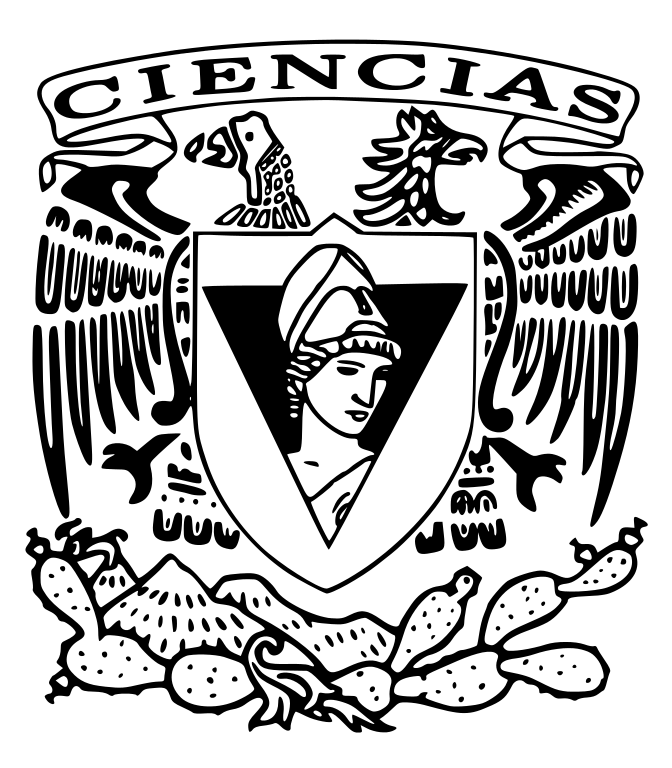
\includegraphics[scale=0.15]{Escudo fac ciencias.png} \textcolor{white}{FFFACULTAD DE CIENCIAS UNAMMM} 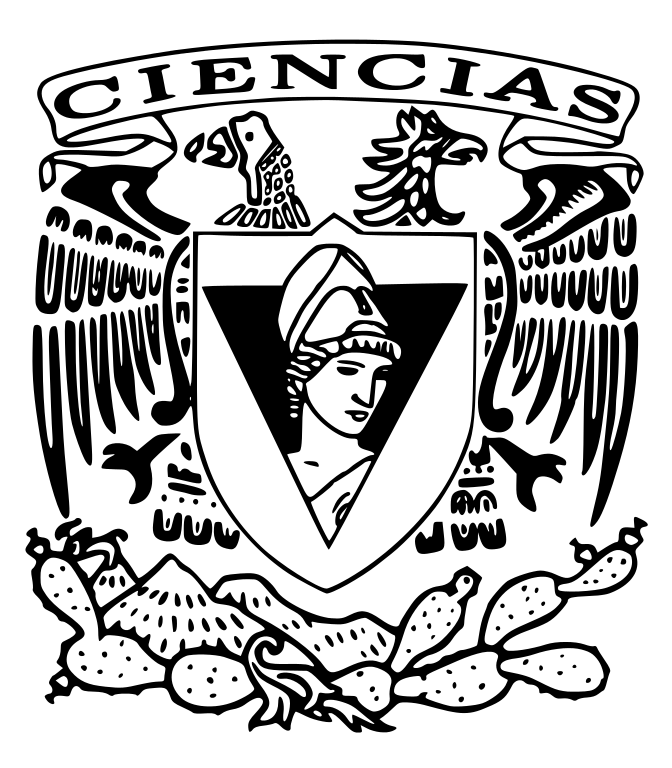
\includegraphics[scale=0.15]{Escudo fac ciencias.png}
\end{center}

\vspace{-3cm}
\begin{center}
    {\large{{\textsc{Facultad de ciencias UNAM}}}}
\end{center}

%-----------------------------------------------------------|||||||||||||||||||| ---INTEGRANTES--- |||||||||||||||||||||

\vspace{2.5cm}
\hspace{-0.75cm} {\Large{\textbf{Integrantes del equipo:}}}\\

\begin{itemize}
    \item {\Large{Archundia Juárez Adrián}}
    \item {\Large{Duarte Martínez Jordán Aarón}}
    \item {\Large{Nayeli Rodriguez Vega}}
\end{itemize}

\vspace{0.8cm}
\begin{center}

\includegraphics[scale=0.25]{Escudo UNAM.png}
\end{center}

%-----------------------------------------------------------|||||||||||||||| ---FECHA DE ELABORACIÓN--- ||||||||||||||||

\vspace{0.8cm}
\hspace{-0.75cm} {\large{Elaborado el 16 de Noviembre del 2022}}

\newpage



%-----------------------------------------------------------|||||||||||||||||||||| ---RESUMEN--- |||||||||||||||||||||||

\pagestyle{fancy}
        \fancyhf{}
        \rhead{\thepage}
        \lhead{\textsc{Resumen}}

\begin{abstract}
    \Blindtext
\end{abstract}

\newpage

%-----------------------------------------------------------|||||||||||||||||||| ---INTRODUCCIÓN--- ||||||||||||||||||||

\pagestyle{fancy}
        \fancyhf{}
        \rhead{\thepage}
        \lhead{\textsc{Introducción}}

\section*{Introducción}

\begin{multicols}{2}
    \Blindtext
\end{multicols}

\newpage

%-----------------------------------------------------------|||||||||||||| ---DESARROLLO EXPERIMENTAL--- |||||||||||||||

\pagestyle{fancy}
        \fancyhf{}
        \rhead{\thepage}
        \lhead{\textsc{Desarrollo experimental}}

\section*{Desarrollo experimental}

\begin{multicols}{2}
    \Blindtext
\end{multicols}

\newpage

%-----------------------------------------------------------||||||||||||||||||||| ---RESULTADOS--- |||||||||||||||||||||

\pagestyle{fancy}
        \fancyhf{}
        \rhead{\thepage}
        \lhead{\textsc{Resultados}}

\section*{Resultados}

\begin{multicols}{2}
    \Blindtext
\end{multicols}

\newpage

%-----------------------------------------------------------||||||||||||||| ---ANÁLISIS DE RESULTADOS--- |||||||||||||||

\pagestyle{fancy}
        \fancyhf{}
        \rhead{\thepage}
        \lhead{\textsc{Análisis de resultados}}

\section*{Análisis de resultados}

\begin{multicols}{2}
    \Blindtext
\end{multicols}

\newpage

%-----------------------------------------------------------|||||||||||||||||||| ---CONCLUSIONES--- ||||||||||||||||||||

\pagestyle{fancy}
        \fancyhf{}
        \rhead{\thepage}
        \lhead{\textsc{Conclusiones}}

\section*{Conclusiones}

\begin{multicols}{2}
    \Blindtext
\end{multicols}

\newpage

%-----------------------------------------------------------|||||||||||||||||||| ---BIBLIOGRAFIA--- ||||||||||||||||||||

\pagestyle{fancy}
        \fancyhf{}
        \rhead{\thepage}
        \lhead{\textsc{Referencias}}

Aquí las citas porque no se como hacer que aparezcan en printbibliography sin que hayan sido citadas antes, aunque no se preocupe profe, en una práctica real los citaré en otras partes del documento para que así no estén acá de forma bien xd. \cite{Articulo}; \cite{Ariculo_de_memorias_de_un_congreso}; \cite{Cuando_el_resto_falla}; \cite{Documentacion_tecnica}; \cite{Documento_inedito_o_no_formalmente_publicado}; \cite{Informe_publicado_por_una_institucion}; \cite{Libro_con_editorial}; \cite{Libro_sin_editorial}; \cite{Parte_de_un_libro}; \cite{Tesis_de_maestria}; \cite{Tesis_de_doctorado}; \cite{Memorias_De_un_congreso}; \cite{Parte_cap_propio_de_un_libro}.

\printbibliography

\end{document}